\chapter{Információs technológiai infrastruktúrák}
\section{A klasszikus IT infrastruktúra}
\section{Felhőalapú infrastruktúrák}
\subsection{Mi is az a ,,számítási felhő''?}

A ,,számítási felhő'' (angolul \foreignlanguage{english}{cloud computing}) egy modell kényelmes, hálózaton keresztül hozzáférhető, konfigurálható számítási erőforrások (pl. hálózat, szerverek, tárhelyek, alkalmazások és szolgáltatások) egy megosztott készletének elérhetőségére, mely erőforrásokat minimális intézkedési erőfeszítéssel vagy szolgáltatói közbenjárással gyorsan rendelkezésre lehet bocsátani.

\todo{Lehet, hogy még finomítani kell a fordításon!}

\begin{comment}
Cloud computing is a model for enabling ubiquitous, convenient, on-demand network access to a shared pool of configurable computing resources (e.g., networks, servers, storage, applications, and services) that can be rapidly provisioned and released with minimal management effort or service provider interaction. 
\end{comment}

\todo{Forrás: http://csrc.nist.gov/publications/nistpubs/800-145/SP800-145.pdf}
\begin{comment}
The NIST Definition of Cloud Computing
Peter Mell 
Timothy Grance
September 2011
\end{comment}

Felhőként hivatkozhatunk az Interneten keresztül szolgáltatott alkalmazásokra és a hardverre, szoftverre, amelyek ezeket az alkalmazásokat elérhetővé teszik.

\begin{figure}[h!]
\centering
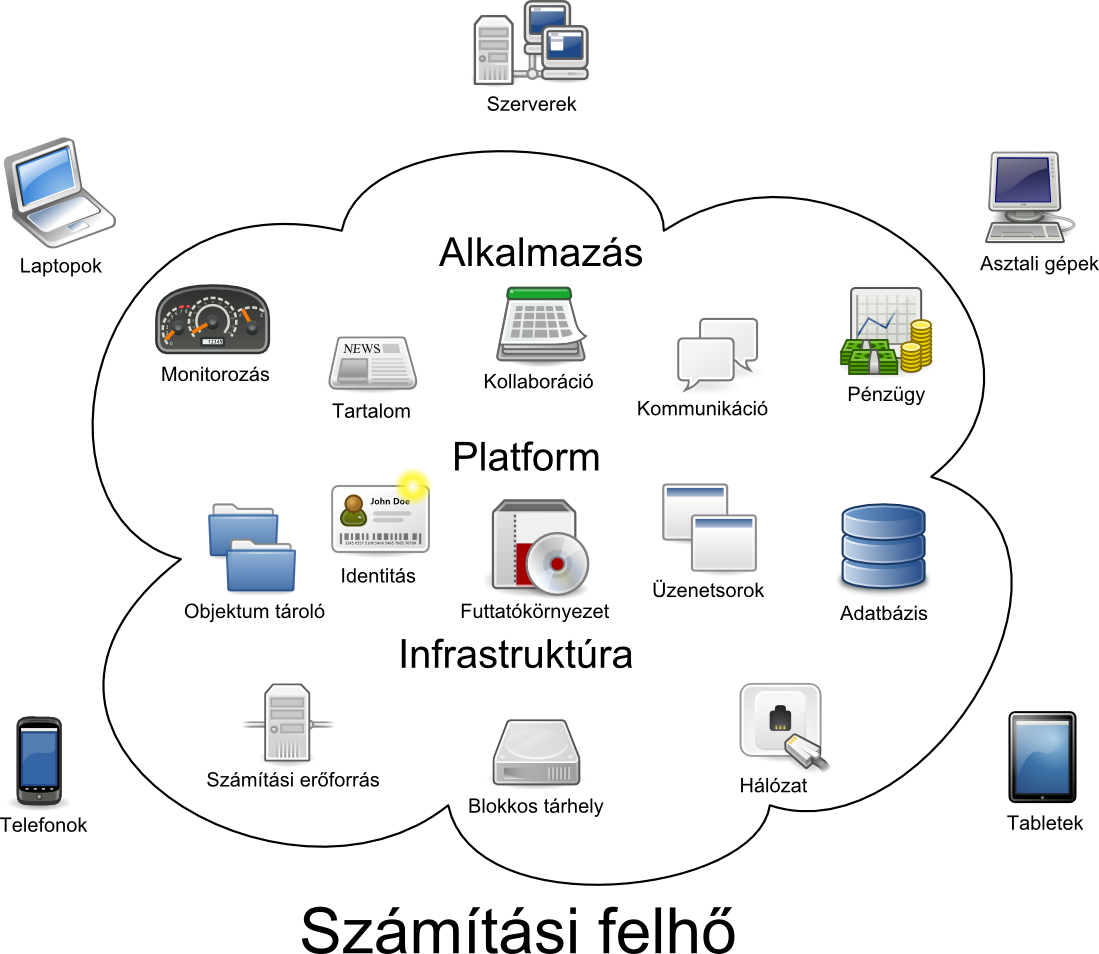
\includegraphics[width=1.0\textwidth]{figures/Cloud_computing_hu.png}
\caption{A számítási felhő (\foreignlanguage{english}{cloud computing})} \label{fig:cloud_computing_hu}
\end{figure}

\todo{Object Storage ?= Objektum tároló}
\todo{Queue ?= Üzenetsorok}
\todo{Runtime ?= Számításelosztás}

